% Options for packages loaded elsewhere
\PassOptionsToPackage{unicode}{hyperref}
\PassOptionsToPackage{hyphens}{url}
%
\documentclass[
]{article}
\usepackage{lmodern}
\usepackage{amssymb,amsmath}
\usepackage{ifxetex,ifluatex}
\ifnum 0\ifxetex 1\fi\ifluatex 1\fi=0 % if pdftex
  \usepackage[T1]{fontenc}
  \usepackage[utf8]{inputenc}
  \usepackage{textcomp} % provide euro and other symbols
\else % if luatex or xetex
  \usepackage{unicode-math}
  \defaultfontfeatures{Scale=MatchLowercase}
  \defaultfontfeatures[\rmfamily]{Ligatures=TeX,Scale=1}
\fi
% Use upquote if available, for straight quotes in verbatim environments
\IfFileExists{upquote.sty}{\usepackage{upquote}}{}
\IfFileExists{microtype.sty}{% use microtype if available
  \usepackage[]{microtype}
  \UseMicrotypeSet[protrusion]{basicmath} % disable protrusion for tt fonts
}{}
\makeatletter
\@ifundefined{KOMAClassName}{% if non-KOMA class
  \IfFileExists{parskip.sty}{%
    \usepackage{parskip}
  }{% else
    \setlength{\parindent}{0pt}
    \setlength{\parskip}{6pt plus 2pt minus 1pt}}
}{% if KOMA class
  \KOMAoptions{parskip=half}}
\makeatother
\usepackage{xcolor}
\IfFileExists{xurl.sty}{\usepackage{xurl}}{} % add URL line breaks if available
\IfFileExists{bookmark.sty}{\usepackage{bookmark}}{\usepackage{hyperref}}
\hypersetup{
  hidelinks,
  pdfcreator={LaTeX via pandoc}}
\urlstyle{same} % disable monospaced font for URLs
\usepackage[margin=1.0in]{geometry}
\usepackage{graphicx}
\makeatletter
\def\maxwidth{\ifdim\Gin@nat@width>\linewidth\linewidth\else\Gin@nat@width\fi}
\def\maxheight{\ifdim\Gin@nat@height>\textheight\textheight\else\Gin@nat@height\fi}
\makeatother
% Scale images if necessary, so that they will not overflow the page
% margins by default, and it is still possible to overwrite the defaults
% using explicit options in \includegraphics[width, height, ...]{}
\setkeys{Gin}{width=\maxwidth,height=\maxheight,keepaspectratio}
% Set default figure placement to htbp
\makeatletter
\def\fps@figure{htbp}
\makeatother
\setlength{\emergencystretch}{3em} % prevent overfull lines
\providecommand{\tightlist}{%
  \setlength{\itemsep}{0pt}\setlength{\parskip}{0pt}}
\setcounter{secnumdepth}{-\maxdimen} % remove section numbering
\usepackage{helvet}
\renewcommand*\familydefault{\sfdefault}
\usepackage{setspace}
\doublespacing
\usepackage[left]{lineno}
\linenumbers
\ifluatex
  \usepackage{selnolig}  % disable illegal ligatures
\fi

\author{}
\date{\vspace{-2.5em}}

\begin{document}

\hypertarget{amplicon-sequence-variants-should-not-replace-operational-taxonomic-units-in-marker-gene-data-analysis}{%
\section{Amplicon sequence variants should not replace operational
taxonomic units in marker-gene data
analysis}\label{amplicon-sequence-variants-should-not-replace-operational-taxonomic-units-in-marker-gene-data-analysis}}

\vspace{20mm}

\textbf{Running title:} ASVs vs.~OTUs

\vspace{20mm}

Patrick D. Schloss\({^\dagger}\)

\vspace{40mm}

\({\dagger}\) To whom corresponsdence should be addressed:

\href{mailto:pschloss@umich.edu}{pschloss@umich.edu}

Department of Microbiology \& Immunology

University of Michigan

Ann Arbor, MI 48109

\vspace{20mm}

\textbf{Observation Format}

\newpage

\hypertarget{abstract-250-words}{%
\subsection{Abstract (250 words)}\label{abstract-250-words}}

\hypertarget{importance-150-words}{%
\subsection{Importance (150 words)}\label{importance-150-words}}

\newpage

16S rRNA gene sequencing is a very powerful technique for describing and
comparing microbial communities. Efforts to link 16S rRNA gene sequences
to taxonomic levels based on distance thresholds go back to at least the
1990s. The distance-based thresholds that were developed and are now
widely used (3\%) were based on DNA-DNA hybridization approaches that
are not as precise as genome sequencing. Instead, genome sequencing
technologies have suggested that the widely used 3\% distance threshold
to operationally define bacterial taxa is too coarse. As an alternative
to OTUs, amplicon sequencing variants (ASVs) have been proposed as a way
to adopt the thresholds suggested by genome sequencing to microbial
community analysis using 16S rRNA gene sequences. ASVs are a unit of
microbial community inference that do not cluster sequences based on a
distance-based threshold. However, most bacterial genomes have more than
1 copy of the rrn operon and those copies are not identical. Therefore,
using too fine a threshold to identify OTUs creates the risk of
splitting a single genome into multiple bins and using too broad of a
threshold to define OTUs creates the risk of lumping together bacterial
species into the same OTU. An example of both is seen in the comparison
of \emph{Staphylococcus aureus} (NCTC 8325) and \emph{S. epidermidis}
(ATCC 12228) where each genome has 5 copies of the 16S rRNA gene. The 10
copies of the 16S rRNA gene each have a different sequence and so if
OTUs are defined based on ASVs, each genome would be split into 5 OTUs.
Conversely, if the copies were clustered using a 3\% distance threshold
all 10 copies would cluster into the same OTU. The goal of this study
was to quantify the risk of splitting a single genome into multiple bins
and the risk of lumping together different bacterial species into the
same bin.

To investigate the variation in the number of copies of the 16S rRNA
gene per genome as well as the intragenomic variation among copies of
the 16S rRNA gene, I obtained reference 16S rRNA sequences from the rrn
copy number database (rrnDB; CITATION). Among the \textbf{4,774} species
represented in the rrnDB there were \textbf{15,614} genomes. The median
number of rrn operson per species ranged between \textbf{1}
(e.g.~\textbf{\emph{Mycobacterium tuberculosis}}) and \textbf{19}
(\textbf{\emph{Metabacillus litoralis}}) copies of the rrn operon. As
the number of copies of the operon in a genome increased, the number of
variants of the 16S rRNA gene in each genome also increased
(\textbf{FIGURE}). On average, there were \textbf{1} variants per copy
of the full length 16S rRNA gene and an average of \textbf{0.26},
\textbf{0.33}, and \textbf{0.27} variants when considering the V4,
V3-V4, and V4-V5 regions of the gene, respectively. Although a species
tended to have a consistent number of 16S rRNA gene copies per genome,
the number of total variants increased with the number of genomes that
were sampled (\textbf{Figure 1}). For example,
\textbf{\emph{Mycobacterium tuberculosis}} generally only had \textbf{1}
copy of the gene per genome, but across the \textbf{180} genomes that
have been sequenced there were \textbf{11} versions of the gene.
Similarly, a \emph{E. coli} genome typically had \textbf{7} copies of
the 16S rRNA gene with between \textbf{6} and \textbf{10} distinct full
length sequences per genome. Across the \textbf{958} \emph{E. coli}
genomes that have been sequenced, there were \textbf{1,013} different
variants of the gene. These observations highlight the risk of selecting
a threshold for defining units of inference that is too narrow because
it is possible to split a single genome into multiple units.

A method to avoid splitting a single genome into multiple units of
inference is to cluster 16S rRNA gene sequences together that are
similar. However, this also increases the risk of lumping together genes
from different species that are similar to each other. Therefore, I
assessed the impact of the threshold used to define clusters of 16S rRNA
genes on the propensity to split a genome apart or to lump species
together. For full length 16S rRNA gene sequences, I found that at a
threshold of \textbf{5.5}\%, 95\% of the species with 7 copies of the
rrn operon would be represented by a single OTU. Similarly, thresholds
of \textbf{2.5}, \textbf{4.0}, and \textbf{3.5}\% were observed for the
V4, V3-V4, and V4-V5 regions, respectively. However, at these
thresholds, multiple species could be represented by the same OTU. At
the highest level of resolution, \textbf{3.6}\% of the species shared a
16S rRNA gene sequence variant with another species when considering
full length sequences and \textbf{14.9}, \textbf{10.2}, and
\textbf{12.0}\% when considering the V4, V3-V4, and V4-V5 regions,
respectively. At the commonly used 3\% threshold, \textbf{25.2}\% of the
species shared an OTU when considering full length sequences and
\textbf{33.0}, \textbf{29.4}, and \textbf{32.2}\% when considering the
V4, V3-V4, and V4-V5 regions, respectively. Given the risk of splitting
a genome into multiple OTUs is more biologically problematic than
lumping species together, larger thresholds are advisable.

To provide a more nuanced approach to selecting a threshold, it would be
useful to to quantify the sensitivity and specificity of characterizing
bacterial species using OTUs defined at different thresholds. I created
confusion matrices for multiple regions of the 16S rRNA gene: true
positives were those cases where two ASVs were joined in the same OTU
and the same species; true negatives were those cases where two ASVs
from different OTUs came from different species; false positives were
those ASVs that joined the same OTU, but were from different species;
and false negatives were those ASVs that joined different OTUs, but were
from the same species. By calculating the sensitivity and specificity
for each threshold and each region of the 16S rRNA gene, I was able to
constuct a receiver operator characteristic curve (ROC). Because the ROC
curve represents a range of possible thresholds and sensitivities and
specificities, I used two metrics to select the best threshold for
defining an OTU. First, I identified the thresholds where the
sensitivity and specificity were most similar to each other. For this
criterion, the best distance thresholds were \textbf{6.0}\% (V1-V9),
\textbf{4.5}\% (V4), \textbf{5.5}\% (V3-V4), and \textbf{4.0}\% (V4-V5).
Second, I identified the distance threshold that resulted in the point
on the ROC curve that was closest to perfect classification. For this
criterion, the best distance thresholds were \textbf{5.5}\% (V1-V9),
\textbf{3.5}\% (V4), \textbf{4.5}\% (V3-V4), and \textbf{3.5}\% (V4-V5).
Surprisingly, these analyses revealed that thresholds near 3\% distance
balance the risks of splitting genomes into separate OTUs and lumping
species into the same OTU.

The results of this analysis demonstrate that there is a significant
risk of splitting single genomes into multiple bins if too fine of a
threshold is applied to defining an OTU. An ongoing problem for
amplicon-based studies is defining a meaningful taxonomic unit of
inference. Since there is no consensus definition for a biological
species concept, microbiologists must accept that how we have named
bacterial species is biased and that taxonomic rules are not applied in
a consistent manner. This makes it more challenging to attempt to fit a
distance threshold to define an OTU definition that matches a set of
species names. Furthermore, it is unlikely that the 16S rRNA gene
evolves at the same rate across all bacterial lineages, which limits the
biological interpretation of a common OTU definition. At best, a
distance-based definition of a taxonomic unit is operational. There is
general agreement in bacterial systematics that to classify something to
a bacterial species, you need phenotypic and genome sequence data
(CITATION). We are asking too much of a short section of a bacterial
genome to be able to differentiate between species. It is difficult to
defend a unit of inference that would split a single genome into
multiple taxonomic units. It is not biologically plausible to entertain
the possability that parts of a genome would have different ecologies.
Although there are multiple reasons that proponents of ASVs encourage
their use, the significant risk of splitting genomes is too high to
warrant their use.

\textbf{Materials and Methods. (i) Data availability.} The 16S rRNA gene
sequences used in this study were obtained from the \emph{rrn}DB
(\url{https://rrndb.umms.med.umich.edu}; version 5.6, released November
8, 2019). At the time of submission, this is the most current version of
the database. The \emph{rrn}DB obtained the curated 16S rRNA gene
sequences from the KEGG database, which ultimately obtained them from
NCBI's non-redundant RefSeq database. The \emph{rrn}DB provides
downloadable versions of the sequences with their taxonomy as determined
using the naive Bayesian classifier trained on the RDP reference
taxonomy. For some genomes this resulted in multiple classifications
since a genome's 16S rRNA gene sequences were not identical. Instead, I
mapped the RefSeq accession number for each genome in the database to
obtain a single taxonomy for each genome. Because strain names were not
consistently given to genomes across bacterial species, the strain level
designations were ignored.

\textbf{(ii) Definition of regions within 16S rRNA gene.} The full
length 16S rRNA gene sequences were aligned to a SILVA reference
alignment of the 16S rRNA gene (v138) using the mothur software package
(v. 1.XX). Regions of the 16S rRNA gene were selected because of their
use in the microbial ecology literature. Full length sequences
corresponded to \emph{E. coli} positions XX through XXXX, V4 to
positions XXX through XXX, V3-V4 to positions XXX through XXX, and V4-V5
to positions XXX through XXX.

\textbf{(iii) Controlling for uneven sampling of genomes by species.}
Because of the uneven distribution of genome sequences across species,
for the analysis of splitting genomes and lumping species I randomly
selected one genome for each species. The random selection was repeated
100 times. Analyses based on this randomization report the median of the
100 randomizations. The intraquartile range between randomizations was
typically less than XXXX. Because it was so small, confidence intervals
are not included in Figure 2.

\textbf{(iv) Reproducible data analysis.} The code to perform the
analysis in this manuscript and its hisotry are available as a git-based
version control repository on GitHub
(\url{https://github.com/pschloss/Schloss_rrnAnalysis_XXXX_2020}). The
analysis can be regenerated using a GNU Make-based workflow that made
use of built-in bash tools (v. 3.2.57), mothur (v. 1.XX), and R (v.
4.X.X). Within R, I used the tidyverse (v. 4.X.X), data.table (v.
4.X.X), Rcpp (v. 4.X.X), furrr (v. 4.X.X), and rmarkdown (v. 4.X.X)
packages. The conception and development of this analysis is available
as a playlist on the Riffomonas YouTube channel
(\url{https://www.youtube.com/playlist?list=PLmNrK_nkqBpKY3SZiivlIGvcLX-KHmfR8}).

\textbf{Acknowledgements.} I am grateful to Robert Hein and Thomas
Schmidt who maintain the rrnDB for their help in understanding the
curation of the database and for making the 16S rRNA gene sequences and
related metadata publicly available. I am also grateful to community
members who watched the serialized version of this analysis on YouTube
and provided their suggestions and questions.

This work was supported, in part, through grants from the NIH to PDS
(P30DK034933, U01AI124255, and R01CA215574).

\newpage

\hypertarget{references}{%
\subsection{References}\label{references}}

\newpage

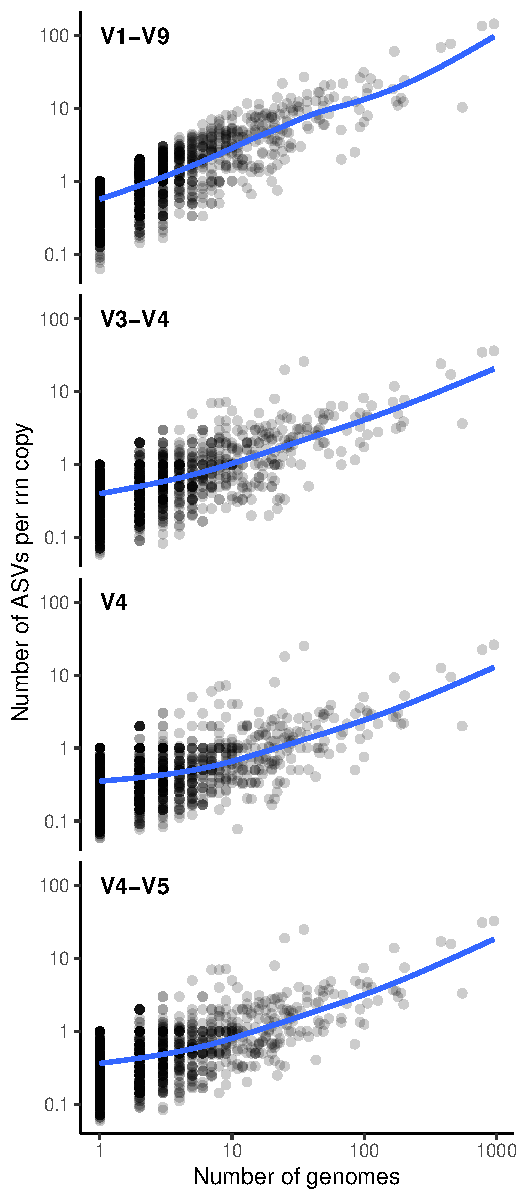
\includegraphics{../figures/esv_rate.pdf}

\textbf{Figure 1. ESV rate increases as the number of genomes sampled
per species increases}

\newpage

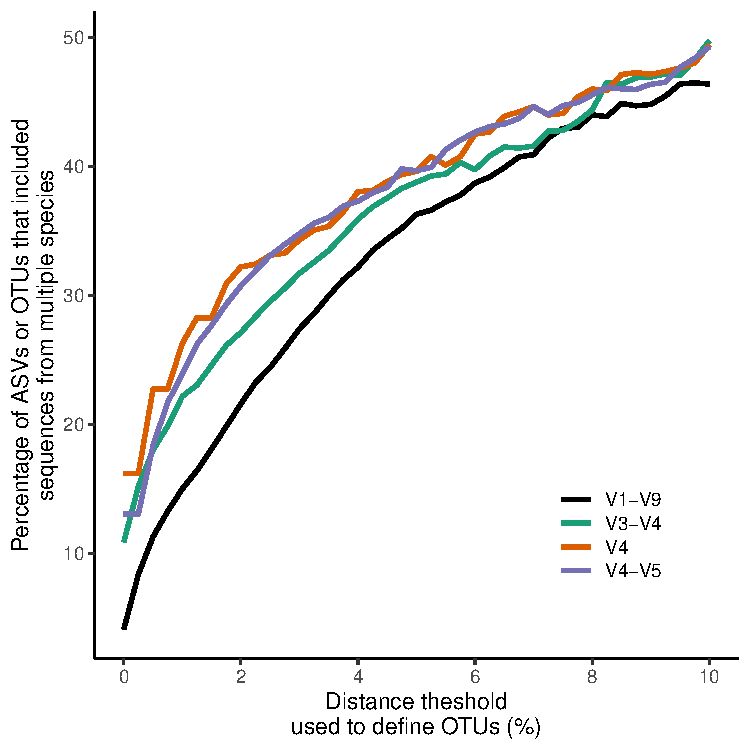
\includegraphics{../figures/lump_split.pdf}

\textbf{Figure 2. Rate of lumping and splitting by distance threshold}

\newpage

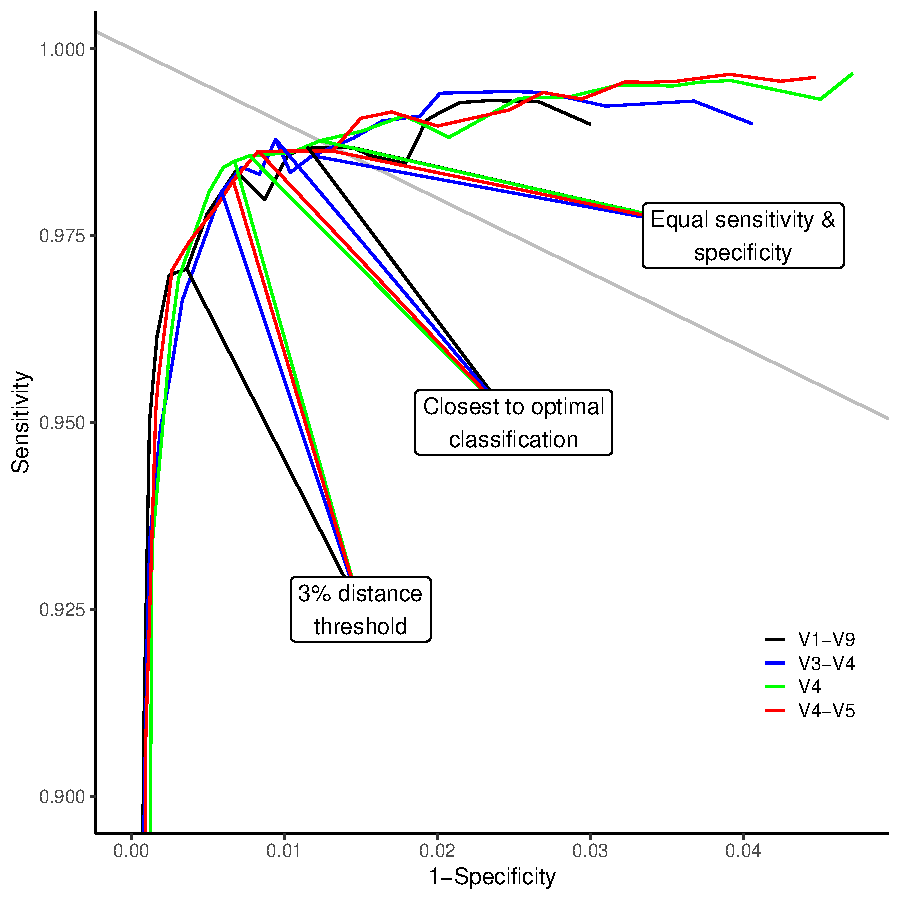
\includegraphics{../figures/roc_curve.pdf}

\textbf{Figure S1. Receiver operator characteristic curve and position
of various thresholds}

\end{document}
